\documentclass[12pt, twoside]{article}
\usepackage[letterpaper, margin=1in, headsep=0.5in]{geometry}
\usepackage[english]{babel}
\usepackage[utf8]{inputenc}
\usepackage{amsmath}
\usepackage{amsfonts}
\usepackage{amssymb}
\usepackage{tikz}
\usetikzlibrary{quotes, angles}
\usepackage{graphicx}
\usepackage{enumitem}
\usepackage{multicol}

\newif\ifmeta
\metatrue %print standards and topics tags

\title{Regents Geometry}
\author{Chris Huson}
\date{December 2021}

\usepackage{fancyhdr}
\pagestyle{fancy}
\fancyhf{}
\renewcommand{\headrulewidth}{0pt} % disable the underline of the header
\raggedbottom

\fancyhead[LE]{\thepage}
\fancyhead[RO]{\thepage \\ Name: \hspace{4cm} \,\\}
\fancyhead[LO]{BECA / Dr. Huson / Geometry 5 Congruence Transformations}

\begin{document}

\subsubsection*{5.7 Classwork: Rotation review \hfill CCSS.HSN.RN.A.2}
\begin{enumerate}
  \item Rotate the triangle $90^\circ$ clockwise around the origin, $\triangle ABC \rightarrow \triangle A'B'C'$. Complete the table of the coordinates and plot and label the image on the grid. \vspace{0.25cm}
  \begin{multicols}{2}
    $A(1,2) \rightarrow$ \\[0.7cm]
    $B(1,4) \rightarrow$ \\[0.7cm]
    $C(4,2) \rightarrow$ \\[0.7cm]
      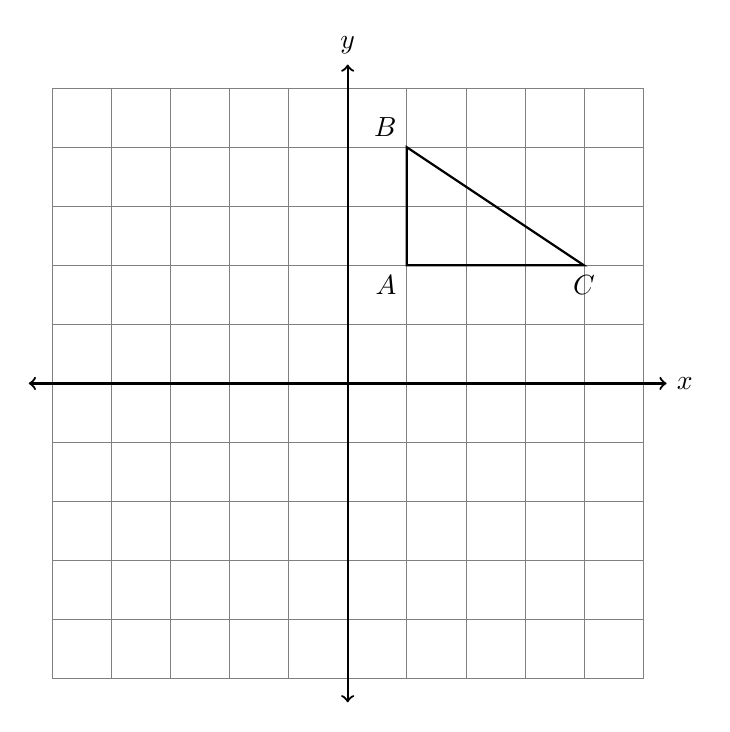
\begin{tikzpicture}[scale=.75]
      \draw [help lines] (-5,-5) grid (5,5);
      \draw [thick, <->] (-5.4,0) -- (5.4,0) node [right] {$x$};
      \draw [thick, <->] (0,-5.4)--(0,5.4) node [above] {$y$};  
      \draw [thick]
        (1,2) node[below left] {$A$}--
        (1,4) node[above left] {$B$}--
        (4,2) node[below] {$C$}--cycle;  
      \end{tikzpicture}
    \end{multicols}
  
    \item $\triangle ABC$ is shown with vertices $A(-1,3)$, $B(4,0)$, and $C(5,3)$. Rotate the triangle $90^\circ$ counter clockwise around the origin. Write down its coordinates in a table and plot and label it on the graph.
  \begin{flushright}
    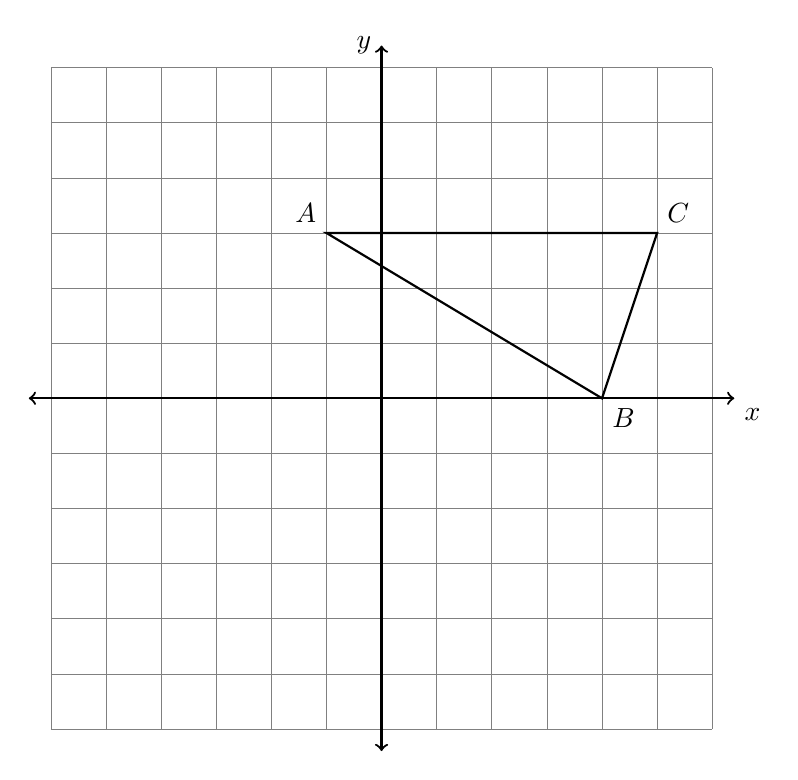
\begin{tikzpicture}[scale=0.7]
      \draw [help lines] (-6,-6) grid (6,6);
      \draw [thick, <->] (-6.4,0) -- (6.4,0) node [below right] {$x$};
      \draw [thick, <->] (0,-6.4)--(0,6.4) node [left] {$y$};
      \draw [thick] (-1,3) node[above left] {$A$}--
        (4,0) node[below right] {$B$}--
        (5,3) node[above right] {$C$}--
        cycle;
    \end{tikzpicture}
    \end{flushright}

\end{enumerate}
\end{document}